\newpage
\lecture{1}{Введение в случайные процессы.}
\section{Введение}
Случайным процессом неформально называем явление, развитие которого во времени
мы не можем однозначно установить.
\\
Например, курсы валют/акций в бытовом смысле случайны; кривая качества обучения
в машинном обучении, сила электрического сигнала, броуновское движение случайно.
\\
Соответственно, мы не можем знать, что с процессом будет точно, но, к примеру,
среднее, диапазон разброса значений, вероятности мы можем установить.
\begin{Def}
    \textbf{Случайным процессом} называется однопараметрическое семейство
    $\left\{ \xi(\omega, t) \mid t \in T \subseteq \RR, \omega \in \Omega
    \right\}$, определенных на одном и том же вероятностном пространстве $\left(
        \Omega, \cF, \PP \right)$. Здесь $\Omega$~--- пространство исходов,
    $\omega$~--- исход, $t$~--- время, $\PP$~--- вероятностная мера, а $\cF$~---
    некоторая $\sigma$-алгебра.
\end{Def}
\begin{Def}
    \textbf{Сечением случайного процесса} называется случайная величина
    $\xi(\omega, t_0)$.
\end{Def}
\begin{Def}
    \textbf{Реализацией (траекторией) случайного процесса} называется
    детерминированная функция $\xi(\omega_0, t)$.
\end{Def}
Пусть даны $n\geq 1$ сечений $\left\{ \xi(\omega, t_i) \right\}_{i=1}^n$, из
которых образован случайный вектор $\left( \xi(\omega, t_1), \xi(\omega, t_2),
    \dots, \xi(\omega, t_n) \right)$.
\begin{Def}
    \textbf{$n$-мерной функцией распределения случайного процесса} называется
    \begin{align*}
      & F_\xi \left( x_1, x_2, \dots, x_n; t_1, t_2, \dots, t_n \right) = \PP\left( \omega : \forall i \in \{1, \dots, n\} \ \xi(\omega, t_i) < x_i \right)
    \end{align*}
\end{Def}
\begin{Def}
    Совокупность функций распределения для всех $n \in \NN$, $t_1, \dots, t_n
    \in T$ называется \textbf{семейством конечномерных распределений случайного
      процесса} $left\{\xi(t): t \in T\}$
\end{Def}
\begin{Def}
    \textbf{Вторичное вероятностное пространство} определяется так.
    \\
    Пусть $X = \left\{ x(t) : D(x) \supseteq T \right\}$, в котором лежат
    траектории процесса $\xi(t)$.
    \\
    Пусть $B_X^T$~--- $\sigma$-алгебра подмножеств $X$, порожденная множествами
    \begin{align*}
      & C = \left\{ x \in X: \forall i \in \{1, \dots, n\} x(t_i) \in B_i \right\}
    \end{align*}
    для всяких $t_1, \dots, t_n \in T$, $B_1, \dots, B_n$~--- борелевских.
    \\
    Пусть вероятность введена как
    \begin{align*}
      & \PP_X(B) = \PP\left( \omega: \xi(\omega, \cdot) \in B \right)
    \end{align*}
    Так определили.
\end{Def}
\textbf{Свойства $n$-мерной функции распределения}
\begin{itemize}
    \item $0 \leq F_\xi \left( x_1, x_2, \dots, x_n; t_1, t_2, \dots, t_n
    \right) \leq 1$.
    \item $F_\xi \left( x_1, x_2, \dots, x_n; t_1, t_2, \dots, t_n \right)$
    непрерывна слева для каждой $x_i$.
    \item Если $\exists x_i \to -\infty$, то $F_\xi \left( x_1, x_2, \dots, x_n;
        t_1, t_2, \dots, t_n \right) \to 0$.
    \item Если $\forall x_i \to \infty$, то $F_\xi \left( x_1, x_2, \dots, x_n;
        t_1, t_2, \dots, t_n \right) \to 1$.
    \item Функции $F_\xi \left( x_1, x_2, \dots, x_n; t_1, t_2, \dots, t_n
    \right)$ монотонны в следующем смысле:
    \begin{align*}
      & \Delta_1 \Delta_2 \dots \Delta_n F_\xi \left( x_1, x_2, \dots, x_n; t_1, t_2, \dots, t_n \right) \geq 0
    \end{align*}
    где $\Delta_i$~--- оператор конечной разности
    \begin{align*}
      & \Delta_i F_\xi \left( x_1, x_2, \dots, x_n; t_1, t_2, \dots, t_n \right) = F_\xi \left( x_1, \dots, x_{i-1}, x_i + h_i, x_{i+1}, \dots, x_n; t_1, t_2, \dots, t_n \right) -\\
      & - F_\xi \left( x_1, \dots, x_{i-1}, x_i, x_{i+1}, \dots, x_n; t_1, t_2, \dots, t_n \right), \ h_i \geq 0
    \end{align*}
    \item Для всякой перестановки $\left(k_1, k_2, \dots, k_n\right)$ индексов
    $\{1, 2, \dots, n\}$ верно
    \begin{align*}
      & F_\xi \left( x_1, x_2, \dots, x_n; t_1, t_2, \dots, t_n \right) = F_\xi \left( x_{k_1}, x_{k_2}, \dots, x_{k_n}; t_{k_1}, t_{k_2}, \dots, t_{k_n} \right)
    \end{align*}
    \item $\forall k \in \{1, \dots, n\}$, $\forall x_1, \dots, x_k \in \RR$
    \begin{align*}
      & F_\xi \left( x_1, x_2, \dots, x_k, +\infty, \dots, +\infty; t_1, t_2, \dots, t_k, t_{k+1}, \dots, t_n \right) = F_\xi \left( x_1, x_2, \dots, x_k; t_1, t_2, \dots, t_k \right)
    \end{align*}   
\end{itemize}
Поясним четвертое свойство.
\begin{align*}
  & \Delta_1 F_\xi \left( x_1; t_1\right) = F_\xi \left( x_1+h_1; t_1\right) - F_\xi \left( x_1; t_1\right) = \PP\left( \xi(t_1) \in [x_1, x_1+h) \right) \geq 0
\end{align*}
\begin{align*}
  & \Delta_1 \Delta_2 F_\xi \left( x_1,x_2; t_1,t_2\right) = \Delta_1\left( F_\xi \left( x_1,x_2+h_2; t_1,t_2\right) - F_\xi \left( x_1,x_2; t_1,t_2\right) \right) = F_\xi \left( x_1,x_2+h_2; t_1,t_2\right) - \\
  & - F_\xi \left( x_1-h_1,x_2+h_2; t_1,t_2\right) - F_\xi \left( x_1+h_1,x_2; t_1,t_2\right) + F_\xi \left( x_1+h_1,x_2; t_1,t_2\right) = \PP\left( \xi(t_1)\in \right. \\
  & \left. \in[x_1, x_1+h_1), \xi(t_2) \in [x_2, x_2+h_2) \right) \geq 0
\end{align*}
% \begin{figure}[h!]
%      \centering
%      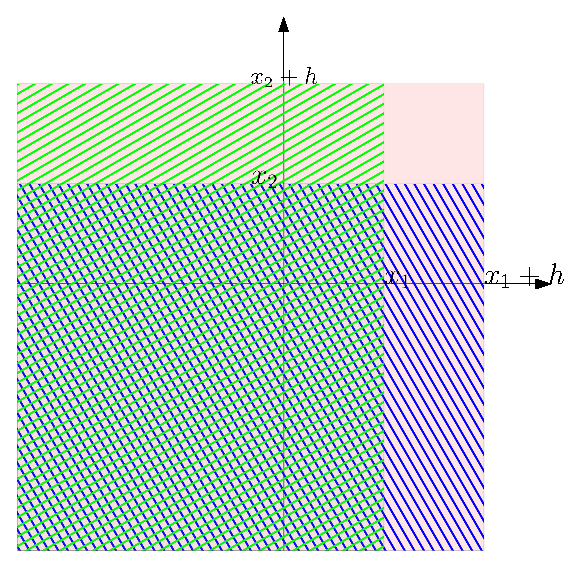
\includegraphics[scale=0.75]{multidim}
%      \label{fig:1.1}
% %     \caption{Перевод единичного круга в $\CC \setminus [-1;1]$}
% \end{figure}
\begin{align*}
  & \Delta_1 \dots \Delta_n F_\xi \left( x_1,\dots, x_n; t_1, \dots, t_n\right) = \PP\left( \xi(t_1)\in [x_1, x_1+h_1), \dots, \xi(t_n) \in [x_n, x_n+h_n) \right) \geq 0
\end{align*}
\begin{theorem} Колмогорова (без доказательства)
    \\
    Пусть задано семейство функций
    \begin{align*}
      & F = \left\{ F \left( x_1,\dots, x_n; t_1, \dots, t_n\right): x_i \in \RR, \ t_i \in T  \right\}
    \end{align*}
    удовлетворяющее условиям, приведенным выше.
    \\
    Тогда существует вероятностное пространство $(\Omega, \cF, \PP)$ и случайный
    процесс $\{\xi(t), t \in T\}$, определенный на нем, такие, что семейство
    конечномерных распределений $F_\xi$ совпадает с $F$.
\end{theorem}
\textbf{Типы процессов по времени}
\begin{itemize}
    \item $\left| T \right| = 1$~--- случайная величина
    \item $\left| T \right| < \infty$~--- случайный вектор
    \item $\left| T \right| = \aleph_0$~--- случайная последовательность
    \item $\left| T \right| > \aleph_0$~--- случайная функция
\end{itemize}
\begin{example}
    Вероятность каких-либо событий не всегда определена. Например,
    \begin{align*}
      & \PP \left( \sup_{t \in [0;1]} \xi(t) \leq x \right) = \PP\left\{ \bigcap_{t \in [0;1]} \left\{ \xi(t) \leq x \right\} \right\}
    \end{align*}
    не событие.
\end{example}
\begin{theorem} Колмогорова о существовании непрерывной модификации (без доказательства)
    \\
    Пусть
    \begin{align*}
      & \left\{ \xi(t) \mid t \in T = [a;b] \right\}
    \end{align*}
    случайный процесс и
    \begin{align*}
      & \exists \alpha > 0, \ \beta > 0, \ c < \infty: \ \forall t, t+h \in [a, b] \ \EE\left| \xi(t+h)-\xi(t) \right|^{\alpha} \leq c \left| h \right|^{1+\beta}
    \end{align*}
    то $\xi(t)$ имеет непрерывную модификацию, то есть существует процесс
    $\eta(t)$, заданный на том же пространстве, такой, что
    \begin{align*}
      & \PP\left( \omega: \ \xi(\omega, t) = \eta(\omega, t) \right) = 1
    \end{align*}
    и почти все траектории непрерывны на $[a,b]$.
\end{theorem}
